%%%%%%%%%%%%%%%%%%%%%%%%%%%%%%%%%%%%%%%%%%
%Copyright (C) 2018-2019 YuZJ Lab.
%使用CC-BY-NC-SA授权。一份完整版本的许可证已位于附录。这个版本原始作者YuZJ,
%邮箱\theafamily@126.com(最后连接于2019年06月20日17:32:17)。
%%%%%%%%%%%%%%%%%%%%%%%%%%%%%%%%%%%%%%%%%%
\section{Copyright 版权}
Copyright \copyright{} 2018-2019 YuZJ Lab. \par
使用CC-BY-NC-SA授权。一份完整版本的许可证已位于附录。这个版本原始作者YuZJ,邮箱\url{theafamily@126.com}(最后连接于2019年06月20日17:32:17)。
\begin{center}\large \bf {\color{red}{对本文档所引起的任何后果不作担保!}}\normalall\end{center}
\section{序}
首先声明一下:在这里提及非自由软件并非我的意愿。作为自由软件的支持者,我当然希望你们使用自由软件。但技术所限,非自由的内容不得不被包括在内。\par
“天覆地载,物号数万,而事亦因之,曲成而不遗。”(来自于《天工开物·序言》)人类在计算机技术上的创造亦是如此。很高兴生活在信息时代(也许马上应改为“数据时代”),国内外优秀的软件都可以被免费或付费地获取以为我们所用。然而“工欲善其事,必先利其器”,对于我们来说,掌握如何高效率地使用计算机是十分重要的。如一位数学教师可用\LaTeX\footnote{\LaTeX 是一个产生于 \TeX 的一个排版系统。它在编辑公式方面十分强大(使用 \AmSTeX 等宏包 ),并且能够胜任巨型文档和复杂的排版任务(如交叉引用、创建索引、管理参考文献资料等等)。它使用“LaTeX Project Public Li­cense (LPPL)”开放源代码,并拥有CTAN(综合的TeX档案库网络,拥有\LaTeX 近乎全部的宏包和使用教程,并存在多个镜像站如TUNA源)(【CTAN: Comprehensive TeX Archive Network】\url{https://www.ctan.org/},最后连接于2019年7月6日21:08:02)的管理组织与tug(\TeX 用户组:【TeX Users Group (TUG)】\url{http://www.tug.org/}(最后连接于2019年7月8日15:05:21))。做一点小小的说明:如果不喜欢完全使用鼠标来编辑公式,当编辑复杂公式时我更倾向于\LaTeX。\LaTeX 更多依赖键盘,但是不是一个所见即所得的软件。就像编写网页一样,你需要“编译”(Compile)\LaTeX 代码才能得到正确的文件。再做一点小小的说明,本文档就是用\LaTeX 编写的。}而不是MS Office \footnote{MS是Microsoft(微软)的缩写,MS Office 是微软公司发布的非自由付费办公套件。相对于\LaTeX ,它最大的优点是所见即所得和具有图形界面。} 来高效地编辑公式或使用Git\footnote{这个一点都不讨厌(Git在英文中有“讨厌的人”意),是一个高效易用的分布式版本控制软件。官方网站\url{https://git-scm.com/}(最后连接于2019年7月6日21:06:04)。}管理自己的论文。因此,为了方便信息化教学的开展,我结合自己的工作经历,不自量力地“年来著书一种”,为希望掌握关于如何高效地使用教室计算机的初级和高级技巧的电教委员或者其余希望提高计算机技能的教师、学生及其他教职人员编写了这份文件。\par
手册中题为“入门”的章节是针对初学者的(前提条件:你需要知道开机按钮在哪里。详情请参阅主机的说明书),它大致介绍了Windows操作系统和MS Office等软件来实现日常教学,Windows操作系统的简单技巧与最基础的Windows安全。题为“进阶”的章节是针对已有一定技能基础并希望尝试更加有效的Windows安全工具(如使用以GNU/Linux\footnote{应该使用“GNU/Linux”而不是“Linux”。请参见【Richard Stallman之GNU/Linux问答】\url{https://www.gnu.org/gnu/gnu-linux-faq.html}(最后连接于2019年06月20日17:32:59)。关于GNU/Linux的详细介绍参见\pageref{sec:gnulinux}页\ref{sec:gnulinux}。}为操作系统的反病毒光盘清除计算机病毒——我暂时不会教你手工杀毒,那是尤金·卡巴斯基\footnote{俄罗斯“卡巴斯基实验室”创立者及董事长。1989年10月的一次手工杀毒(Cascade病毒)激起了他对于计算机反病毒的兴趣并在这方面深度研究,不久即写出反病毒软件并于1997年成立卡巴斯基实验室。目前专注病毒研究。}之类大神干的事)的电教委员的。题为“高级”的章简单地节介绍了GNU/Linux 操作系统的一部分入门知识及其教学实现。\par
在介绍多种多样的软件时,我遵循的原则是法律——性能——易用性——价格。在性能相同的情况下,易用性优先(大多是专有软件),但我也不会忘了推荐一些不错的自由免费软件以减少希望廉价使用正版软件者的开支。通过对自由/开源与专有软件的论证,我希望能够引导学生形成他们的软件价值观。这也是我在本书末尾附上《GNU GPL》的原因。\par
 在使用这份手册时,最重要的是实践。本人才疏学浅,文本中或许有(大量)错误\footnote{尤其是对于GNU/Linux, \LaTeX 排版系统或者VIM等高级文本编辑器 。},请广大读者不吝赐教。联系方式:\url{theafamily@126.com}(最后连接于2019年06月20日17:32:17)。如果文档中存在任何侵权之处,请按邮箱联系。一经确认,将立刻改正。“丐大业文人,弃置案头。此书于功名进取,毫不相关也。”\par
时己亥年肆月廿七日,西历2019年5月1日\par
慈溪YuZJ于家之书房
\section{致班主任}
\noindent 尊敬的班主任:
您好!\par
当你发现你的学生在看这本书时,您不用感到惊慌。本书不会包含任何有关逃避班主任的耳目来玩游戏或者任何类似的技术,也不会让学生沉迷于计算机无法自拔。本书的主要目的是培养能够熟练使用计算机的高级电教委员,我相信在这本书的帮助下,你会对他们的工作更加满意的。\par
这本书里的大部分操作(包括但不限于激活操作系统、激活部分软件、下载软件、更新操作系统以及反病毒软件病毒库)需要网络连接。这些网络连接虽然可以被以其他工作替代,但是这将大大增加电教委员的工作量。因此,在确保电教委员是一个品行优良、作风端正的人的前提下,请允许你的电教委员使用网络连接。如果你们班的学生都是自控能力极强的学生,您可以考虑对这台计算机开放互联网。这样您的学生查询英语单词能够更加方便,计算机系统也能时时保持最新。\par
如果你发现通过使用这本书您的电教委员的效率确实比以往高了不少,你也可以免费从网络上获得一本。我相信这本书中的某些章节对于提高您的生产力将会有所帮助。
\section{重要!预先警告}
\begin{window}[2,r,{\shadowbox{\parbox[t]{6cm}{\footnotesize 以下为对原文中重要内容的引用。火绒工程师认为:所谓的“下载器”和“高速下载通道”既没有用处,也没有存在的必要。为了躲避这些“下载器”的侵扰,用户可以去某个软件的官网下载产品,一般不用担心下载到下载器。这些“下载器”存在的意义就是为了捆绑安装其他软件。这些捆绑软件无一例外都不是用户当时想要的,如果想要这些软件,在下载站上都能找到。总之,除了给用户制造麻烦,所谓这些“高速下载通道”和“下载器”没有任何作用。\normalall}}},{}]
本书内所有网络链接在“最后连接时间”前均有效且已经过Norton Safe Web的Edge插件、Microsoft SmartScreen筛选器及卡巴斯基网络反病毒(包含于卡巴斯基免费版2019,病毒库更新时间为检测当天12:00)检测。 {\color{red}{注意,至少我坚持认为本书中提到的所有应用程序都应该从其官方网站或镜像源处下载。我们不推荐本书的使用者从任何非官方软件发布处\footnote{如腾讯电脑管家“软件中心”(提供过时的软件,如“Avira Antivir Personal 个人免费版”。软件链接:\url{https://pc.qq.com/detail/19/detail_819.html}(最后连接于2019年7月29日16:02:42),软件的发布日期为2016-11-14,最新版本发布日期应该已经是2019了。)或PC6等下载站(请参见【火绒安全-下载站行业乱象:流氓软件和电脑病毒重灾区】\url{https://www.huorong.cn/info/149181215360.html}(最后连接于2019年6月21日16:20:40))。}下载任何本书中提到的软件(官方认可的镜像源除外)。}}。\par 同样需要声明的是,从任何网站下载“破解版”或“注册机”“算号器(KeyGen)”“KMS注册机(这里仅指非法的KMS服务器。合法的服务器不用担心)”(以下简称“侵权程序”)都是不被允许的。这些侵权程序大部分含有“后门”或直接携带病毒(主要表现为网络蠕虫、挖矿机程序和Rootkit,或皆有)。具体请参见【“小马激活”病毒日感染数万台电脑 建议百度、360屏蔽该关键词】\url{https://www.huorong.cn/info/146173867117.html},【“小马激活”病毒新变种分析报告】\url{https://www.huorong.cn/info/146173922919.html},【激活工具带毒感染量近60万 北京等四城市用户不被攻击】\url{https://www.huorong.cn/info/1526627586130.html},【火绒安全警报:病毒伪装成激活工具  强制安装360、2345浏览器】\url{https://www.huorong.cn/info/1535631707148.html}(最后连接于2019年6月21日16:30:28)。\end{window}\par
 对于错误反馈,任何由于违反以上两条原则导致的问题将不会被回复。\par 
 如果你确信你的下载站提供了可靠的软件,你也需要使用哈希校验来确保文件可靠性。方法:使用7Zip在文件资源管理器中的右键菜单“CRC SHA”选项校验哈希值并于官方提供的哈希制作比较。如果一致,那么这个软件可视为是官方的。 \par
  第三点:本书所有操作都是基于硬盘启动(而不是网络启动)的计算机,请先检查一下硬盘并与电教员联系。\par 
  第四点:请注意在安装任何软件时查看最终用户许可声明(EULA)和隐私协定!这将让你了解软件的使用条例。经验主义和机会主义者在将会付出代价。
\begin{center}\Large {\color{red}{本书将不会提供任何有关破解专有软件的方法\\或进行反向工程、反向汇编、反向编译的知识。}\normalall}\end{center}
经检测的镜像站列表如下(检测于2019年6月22日17:16:47):
\begin{description}
	\item [【清华大学开源软件镜像站 | Tsinghua Open Source Mirror】]\url{https://mirrors.tuna.tsinghua.edu.cn/}
	\item [【USTC Open Source Software Mirror】]\url{http://mirrors.ustc.edu.cn/}
	\item [【欢迎访问网易开源镜像站】]\url{http://ubuntu.cn99.com/}\url{http://mirrors.163.com/}
	\item [【华为开源镜像站\_软件开发服务\_华为云】]\url{https://mirrors.huaweicloud.com/}
	\item [【阿里巴巴开源镜像站】]\url{https://opsx.alibaba.com/mirror}
	\item [【兰州大学开源社区镜像站】]\url{http://mirror.lzu.edu.cn/}
	\item [【重庆大学开源软件镜像站 | Chongqing University Open Source Mirror Site】] \url{https://mirrors.cqu.edu.cn/}
	\item [【Nanjing University Open Source Mirror Site】] \url{https://mirrors.nju.edu.cn/}
	\item [【南京邮电大学开源软件镜像站 | Njupt Open Source Mirror】]\url{https://mirrors.njupt.edu.cn/}
	\item [【Mirrors@NWAFU】]\url{https://mirrors.nwafu.edu.cn/}
	\item [【这个似乎是搜狐的......具体叫什么我也不清楚】]\url{https://mirrors.sohu.com/}
	\item [【SourceForge - Download, Develop and Publish Free Open Source Software】] \url{https://sourceforge.net/}
	\item [【FOSSHUB】] \url{https://www.fosshub.com/}
	\item [【The world’s leading software development platform · GitHub】] \url{https://github.com/}
\end{description}
\section{自由软件、开源软件和专有软件}
我们以是否公开源代码为标准来区分一个软件是不是专有软件。不公开源代码(你只能得到可执行文件(参见\pageref{sec:exe}页的\ref{sec:exe}))的软件称为“专有软件”,而公开源代码的软件称为开源或者自由软件。我们以许可证是否兼容《GNU General Public License v3》(《GNU通用公共授权第3版》)来确定这个软件是否自由,如果兼容即为自由软件\footnote{其实完整的标准应该是:源代码允许用户“自由”使用的软件称为自由软件。然而“自由”是一个很难定义的名词,因此我们使用Richard Stallman的标准界定“自由”。请参见【Various Licenses and Comments about Them - GNU Project - Free Software Foundation】\url{http://www.gnu.org/licenses/license-list.html(最后连接于2019年07月30日18:08:02)来确定你的许可证是否自由。}}一个软件在安装时就会展示许可证(如下图为安装Filezilla时展示的GNU GPL许可证),你应该仔细地阅读它并决定是否安装。
\begin{center}
	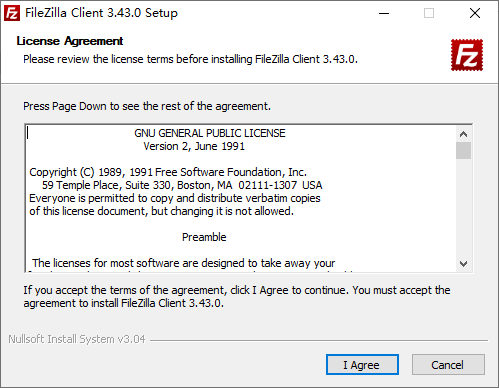
\includegraphics[scale=0.6]{pic/fzi}
\end{center}\par
哪些是专有软件?我们日常所用的软件(如Windows操作系统、Office办公软件、QQ、微信与Photoshop等等),基本上全都是专有软件。\par
我虽然支持自由软件,但是承认拥有\bf 合法版权\normalall 的专有软件的合法性。在这本书中,在\bf 不影响使用\normalall 的前提下如果能完成此功能的专有软件能被自由/开源软件替代,我将使用后者。以下是一些常见问题的解答。
\subsection{为什么本书不使用《GNU GPL》?}
\begin{enumerate}
	\item 第12款规定:“If conditions are imposed on you (whether by court order, agreement or otherwise) that contradict the conditions of this License, they do not excuse you from the conditions of this License.”(意为“即便你面臨與本協議條款衝突的條件(來自於法庭要求、協議或其他),那也不能成為你違背本協議的理由。”)
	\item 2.序言规定:For the developers' and authors' protection, the GPL clearly explains that there is no warranty for this free software. (意为“為了保護每一位作者和開發者,GNU通用公共授權合約指明一點:自由軟體並沒有品質擔保。”)
	\item 存在一些其他的表述不清以及前后矛盾问题。
\end{enumerate}
\subsection{那么,使用自由/开源软件有什么好处?}
首先是价格。自由软件大多数是免费的,开源软件收费也不多,但功能强大的专有软件大部分收费\footnote{请注意,我没有在道德层面上批判收费行为——无论是专有软件还是自由软件的创造者都有权利因\bf 自己的\normalall 创造得到物质上与精神上的回报。}。显然地,自由/开源软件敢于将代码和开发过程\footnote{源代码的版本控制机制,任何对源代码的修改一经保存都可以被查到。}示人,就说明他们有勇气接受全世界软件开发者和用户,尤其是他的竞争对手等人的监督,敢承诺没有任何恶意代码或者后门。自由软件的开发是分布式的,一旦出现任何漏洞,一定会在漏洞散布之前被全世界的程序员修补。专有软件和开源软件大多数是一家公司集中开发的,如果出现问题几乎只能依靠公司解决。专有软件的代码不开放性决定了恶意代码或“后门”能被非常方便地置入代码中。这种恶意代码不是专业的开发者是无法发现的,而发现此类问题的专业的开发者则有可能受制于政治、经济或法律因素无法曝光此类问题(一个程序员怎么可能与训练有素的律师团队对抗?)。除此之外,一小部分专有软件(尤其是某些手机APP)\footnote{请注意,我并没有夸大现象,以偏概全。}都会收集大大超过他们需求的个人信息,这是我们普通消费者出来拒绝使用以外无法阻止的。
\subsection{那么,为什么自由/开源软件还不流行?}
但是,自由/开源软件生产者内部也会因为意见不同而引发争端,专业/非专业的开发并存也是整个自由/开源软件界存在的问题。自由软件相较于能实现相同功能的专有软件操作一般较为繁琐(如LibreOffice与MS Office,GIMP与Photoshop,GNU/Linux与Windows。当然这一点见仁见智)并声明“不提供品质担保”,这使自由软件的使用者局限于专业领域从业人员而不是大众。自由软件在宣传上显然也弱于专有软件。